\chapter{Математическая статистика}

\section{Основные понятия выборочной теории}

\subsection{Основные определения}

\textbf{Теория вероятностей} -- является разделом <<чистой>> математики,
который строится дедуктивно, исходя из вполне определенного
набора аксиом.

\textbf{Математическая статистика} -- раздел <<прикладной>> математики,
который строится индуктивно: от наблюдений к гипотезе; при этом
аргументация основана на выводах теории вероятностей.

\begin{table}[H]
    \centering
    \begin{tabular}{|l|l|}
        \hline
        Типовая задача ТВ & Типовая задача МС \\
        \hline
        1) при подбрасывании монеты & Известно, что после $n$ \\
        вероятность выпадения герба & подбрасываний монеты герб \\
        равна $p$. Какова вероятность & выпал $m$ раз. Чему равна \\
        того, что после $n$ подбрасываний & вероятность выпадения герба \\
        герб выпадет $m$ раз? & в отдельном испытании? \\
        \hline
        2) Закон распределения случайной & После $n$ наблюдений за \\
        величины $X \sim N(m, \sigma^2)$. & реализациями случайной \\
        Какова вероятность того, что & величины $X$ получены значения \\
        $\{ X \in [a,b] \}$ & $x_1, ...x_n$. Какой закон распределения \\
                            & имеет случайная величина $X$? \\
        \hline
    \end{tabular}
\end{table}

\textbf{Основная задача МС} -- разработка методов получения
научно-обоснованных выводов о массовых процессах или явлениях
по результатам наблюдений или экспериментов. При этом указанные выводы
относятся не к отдельным экспериментам, а являются утверждениями о
вероятностых характеристиках изучаемого явления.

Одной из <<общих>> задач математической статистики является следующая
задача: $X$ -- случайная величина, закон распрееления которой
неизвестен. Требуется по результатам наблюдений <<найти>> закон
распределения случайной величины $X$. У этой задачи есть две модификации:

\begin{enumerate}
    \item \textbf{1-я основная задача MC}: закон распределения случайной
        величины $X$ неизвестен вообще; требуется его <<найти>>
    \item \textbf{2-я основная задача МС}: известен общий вид закона
        распределения случайной величины $X$, однако неизвестны значения
        одного или нескольких параметров этого закона. Требуется
        оценить значения неизвестных параметров
\end{enumerate}

\begin{example}
    Пусть $X \sim N(m, \sigma^2)$, где значения $m$, $\sigma^2$
    неизвестны. Требуется оценить $m$ и $\sigma$.
\end{example}

\begin{defenition}
    Пусть $X$ -- случайная величина, закон распределения которой
    неизвестен или известен не полностью

    Множество всех возмоных значений случайной величины $X$ называется
    \textbf{генеральной совокупностью}
\end{defenition}

\begin{defenition}
    \underline{Случайной} выборкой объема $n$ из генеральной совокупности
    $X$ называется случайный вектор

    \begin{equation*}
        \vec X = (X_1, ..., X_n)
    \end{equation*}

    где

    \begin{enumerate}
        \item Случайные величины $X_i, i = \overline{1;n}$ независимы
            в совокупности
        \item $X_i \sim X, i = \overline{1;n}$ ($X_i$ имеет то же
            распределение, что и $X$)
    \end{enumerate}
\end{defenition}

\begin{defenition}
    \underline{Выборкой} объема $n$ из генеральной совокупности $X$
    называется (любая) реализация случайной выборки $X$
\end{defenition}

\begin{note}
    \begin{enumerate}
        \item На практике в результате наблюдений (экспериментов)
            исследователь получает реализацию $\vec x$ -- числовой
            вектор. Сkучайная выборка $\vec X$ используется для
            теоретических рассуждений
        \item Пусть $F(t)$ -- функция распределения случайной
            величины $X$. Тогда

             \begin{equation*}
                F_{\vec X} (t_1, ..., t_n) =
                F(t_1) \cdot F(t_2) \cdot ... \cdot F(t_n)
            \end{equation*}

            -- функция распределения выборки из генеральной
            совокупности $X$
    \end{enumerate}
\end{note}

\begin{defenition}
    Множество всех возможных значений выборки $\vec X$ называется
    выборочным пр-вом и обозначатеся $\mathcal X_n$
\end{defenition}

\begin{defenition}
    Любую функцию $g(\vec X)$ случайной выборки $\vec X$ называется
    статистикой или выборочной характеристикой. Закон распределения
    случайной величины $g(\vec X)$ называется выборочным законом
    распределения
\end{defenition}

\begin{note}
    \begin{enumerate}
        \item Значение $g(\vec x)$ статистики $g$ на выборке $\vec x$
            называется выборочным законом этой статистики
        \item Пусть $\vec x = (x_1, ..., x_n)$ -- реализация выборки
            $\vec X$. Это позволяет считать, что закон распределения
            случайной величины $X$ моделируется дискретной
            случайной величиной, закон распределения которой задан
            таблицей

            \begin{table}[H]
                \centering
                \begin{tabular}{|c||c|c|c|c|c|c|}
                    \hline
                    Значение & $x_1$ & $x_2$ & ... & $x_i$ & ... & $x_n$ \\
                    \hline
                    $P$ & $\frac{1}{n}$ & $\frac{1}{n}$ & ... & $\frac{1}{n}$ & ... & $\frac{1}{n}$ \\
                    \hline
                \end{tabular}
            \end{table}

            ФОТО
    \end{enumerate}
\end{note}

\begin{defenition}
    Выборочным средним (выборочным математическим ожиданием называется
    статистика

    \begin{equation*}
        \hat m(\vec X) = \frac{1}{n} \sum_{i=1}^n X_i
    \end{equation*}

    которая обозначается $\hat m = \overline{X}$
\end{defenition}

\begin{defenition}
    Выборочной дисперсией называют статистику

    \begin{equation*}
        \hat \sigma^2 (\vec X) = \frac{1}{n} \sum_{i=1}^n (X_i - \overline X)^2
    \end{equation*}
\end{defenition}

\begin{defenition}
    Выборочным начальным моментом порядка $j$ называют статистику

    \begin{equation*}
        \hat m_j (\vec X) = \frac{1}{n} \sum_{i=1}^n X_i^j
    \end{equation*}
\end{defenition}

\begin{defenition}
    Центральным выборочным моментом порядка $j$ называют статистику

    \begin{equation*}
        \nu_j (\vec X) = \frac{1}{n} \sum_{i=1}^n (X_i - \overline X)^j
    \end{equation*}
\end{defenition}

ФОТО

\subsection{Предварительная обработка результатов эксперимента}

\subsubsection{Вариационный ряд}

Пусть $\vec x$ -- выборка из генеральной совокупности $X$,

\begin{equation*}
    \vec x = (x_1, ..., x_n)
\end{equation*}

Расположим значения $x_1,...,x_n$ в порядке неубывания

\begin{equation*}
    x_{(1)} \le x_{(2)} \le ... \le x_{(n)} (*)
\end{equation*}

где $x_{(i)}$ -- $i$-й элемент полученной последовательности

\begin{defenition}
    Последовательность значений $x_{(1)},...,x_{(n)}$, удовлетворяющее
    (*), называют вариационным рядом выборки $\vec x$, $x_{(i)}$
    называют $i$-м членом вариационного ряда
\end{defenition}

\begin{defenition}
    Вариационным рядом, отвечащим случайной выборке $\vec X$, называется
    последовательность случайных величин

    \begin{equation*}
        X_{(1)},...,X_{(n)},
    \end{equation*}

    где случайная величина $X_{(i)}$ для каждой реализации $\vec x$
    случайной выборки $\vec X$ принимает значение $x_{(i)}$, равное
    значению $i$-го числа вариационного ряда выборки
    $\vec x, i=\overline{1;n}$
\end{defenition}

\begin{note}
    \begin{enumerate}
        \item
            \begin{equation*}
                P\{ X_{(i)} \le X_{(i+1)} \} = 1
            \end{equation*}

        \item
            \begin{equation*}
                F_{X_{(n)}}(t) = P\{ X_{(n)} < t \} = P\{ X_1 < t,... X_n < t \} = F(t) \cdot ... \cdot F(t) = \big[ F(t) \big]^n
            \end{equation*}

            где $F$ - функция распределения случайной величины $X$

        \item
            \begin{equation*}
                F_{X_(1)}(t) = P\{ X_{(1)} < t \} = 1 - P\{ X_{(1)} \geq t \} = 1 - P\{ X_1 \geq t, ..., X_n \geq t\} = 1 - \big[ 1 - F(t) \big]^n
            \end{equation*}
    \end{enumerate}
\end{note}

\subsubsection{Статистический ряд}

Среди элементво выборки $\vec x$ могут встречаться одинаковые.
Предположим, что среди значений $x_1, ..., x_n$ выделены $m$
попарно различных значений $z_{(1)} < ... < z_{(m)}$, причем
каждый элемент $x_i$ совпадает с некоторым
$z_{(j)}$. Эти значения группируют в таблицу, которая называется
\textbf{статистическим рядом выборки $\vec x$}.

\begin{table}[H]
    \centering
    \begin{tabular}{|c|c|c|c|c|}
        \hline
        $z_{(1)}$ & ... & $z_{(i)}$ & ... & $z_{(m)}$ \\
        \hline
        $n_1$ & ... & $n_i$ & ... & $n_m$ \\
        \hline
    \end{tabular}
\end{table}

Здесь $n_i$ -- число элементов выборки $\vec x$, которые равны
$z_{(i)}$

\begin{note}
    \begin{equation*}
        \sum_{i=1}^m n_i = n
    \end{equation*}
\end{note}

\begin{defenition}
    Число $n_i$ называется частотой значения $z_{(i)}$, а
    величина $\frac{n_i}{n}$ -- относительной частотой этого
    значения.
\end{defenition}

\subsubsection{Эмпирическая функция распределения}

Пусть $\vec x = (x_1, ..., x_n)$ -- выборка из генеральной
совокупности $X$. Обозначим $n(x, \vec x)$ -- число элементов вектора
$\vec x$, которые имеют значения меньше $x$.

\begin{defenition}
    Эмпирической функцией распределения называют функцию

    \begin{equation*}
        F_n : \mathcal R \to \mathcal R
    \end{equation*}

    определенную условием

    \begin{equation*}
        F_n(x) = \frac{n(x, \vec x)}{n}
    \end{equation*}
\end{defenition}

\begin{note}
    \begin{enumerate}
        \item $F_n$ обладает всеми свойствами функции распределения
        \item $F_n$ кусочно-постоянна и скачкообразно изменяет
            свои значения в точке $z_{(i)}$
        \item Если все элементы выборки $\vec x$ попарно различны, то

            \begin{equation*}
                F_n(x) =
                \begin{cases}
                    0, x \le x_{(1)} \\
                    \frac{1}{n}, x_{(1)} < x \le x_{(2)} \\
                    ... \\
                    \frac{i}{n}, x_{(i)} < x \le x_{(i+1)},
                    i = \overline{1; n-1} \\
                    ... \\
                    1, x > x_{(n)} \\
                \end{cases}
            \end{equation*}

        \item Эмпирическая функция распределения $F_n(x)$ позволяет
            интерпретировать выборку $\vec x$ как реализацию дискретной
            случайной величины $\tilde X$, реализация которой имеет вид

            \begin{table}[H]
                \centering
                \begin{tabular}{|c||c|c|c|}
                    \hline
                    $\tilde X$ & $z_{(1)}$ & ... & $z_{(m)}$ \\
                    \hline
                    $P$ & $\frac{n_1}{n}$ & ... & $\frac{n_m}{n}$ \\
                    \hline
                \end{tabular}
            \end{table}

            В дальнейшем это позволит рассматривать численные
            характеристики случайной величины $\tilde X$
            как приближенные
            значения численных характеристик случайной величины $X$.
    \end{enumerate}
\end{note}

\subsubsection{Выборочная функция распределения}

Пусть $\vec X = (X_1, ...,, X_n)$ -- случайная выборка из генеральной
совокупности $X$.

Обозначим $n(x, \vec X)$ -- случайная величина, которая для каждой
реализации $\vec x$ случайной выборки $\vec X$ принимает значение,
равное $n(x, \vec x)$

\begin{defenition}
    Выборочной функцией распределения называется функция

    \begin{equation*}
        \hat F (x, \vec X) = \frac{n(x, \vec X)}{n}
    \end{equation*}
\end{defenition}

\begin{note}
    \begin{enumerate}
        \item При каждом фиксированном $x \in \mathcal R$ функция
            $\hat F_n$ может принимать лишь значения из множества

            \begin{equation*}
                0, \frac{1}{n}, \frac{2}{n}, ..., \frac{n-1}{n}, 1
            \end{equation*}

            Обозначим $p = P \{ X_i < x \}$ ($x \in \mathcal R$
            некоторое фиксированное значение). Величина $p$ не зависит
            от $i$, так как все $X_i$ одинаково распределены. Тогда,
            для любого фиксированного $x \in \mathcal R$

            \begin{equation*}
                P \{ \hat F \big( x, \vec X \big)\} = \frac{k}{n} =
                P\{ n \big(x, \vec X \big) = k \} =
            \end{equation*}

            Так как $X_i$ не только одинаково распределены, но и
            независимы, то указанная вероятность равно вероятности
            поялвения ровно $k$ успехов в серии из $n$ испытаний
            по схеме Бернулли, где успех -- событие $\{ X < x\}$

            \begin{equation*}
                C_n^k p^k q^{n-k},
            \end{equation*}

            где $p = P\{X_i < x \} = P\{X < x\}$, $q = 1 - p$. Таким
            образом для каждого фиксированного $x$ случайная величина
            $Y = n \big(x, \vec X\big)$ имеет распределение
            $Y \sim B(n, p)$
    \end{enumerate}
\end{note}

\begin{theorem}
    Для любого $x \in \mathcal R$ последовательность
    $\hat F_n \big( x, \vec X \big)$ при $x \to \infty$ сходится
    по вероятности к значению $F(x)$, где $F$ - теоретическая
    (<<истинная>>) функция распределения случайной величины $X$, то
    есть

    \begin{equation*}
        \hat F_n \big(x, \vec X\big)  \xrightarrow[n \to \infty]{P} F(x)
    \end{equation*}
\end{theorem}

Доказательство

При каждом фиксированном $x \in \mathcal R$ величина
$\hat F_n \big( x, \vec X \big)$ равна относительной (наблюденной)
частоте успеха в серии из $n$ испытаний с вероятностью успеха
$p = P\{X < x\}$ (см. замечание). Из ЗБЧ в форме Бернулли следует,
что

\begin{equation*}
    \hat F_n \big( \underbrace{x}_\text{наблюденная частота},
    \vec X \big) \xrightarrow[n \to \infty]{P}
    \underbrace{p}_\text{теоретическая частота} = P\{X<x\} = F(x)
\end{equation*}

\subsubsection{Интервальный статистический ряд}

Пусть $\vec x$ -- выборка из генеральной совокупности $X$. Если
объем $n$ этой выборки велик $(n \geq 50)$, то значения $x_i$
группируют не только в статистический ряд, но и в так называемый
\textbf{интервальный статистический ряд}. Для этого отрезок
$J = [x_{(1)}, x_{(n)}]$ делят на $p$ равновеликих частей:

\begin{equation*}
    J_i = [a_i, a_{i+1}), i = \overline{0; p - 1}
\end{equation*}

\begin{equation*}
    J_p = [a_{p-1}, a_p],
\end{equation*}

где $a_i = x_{(1)} + i\Delta, i = \overline{0;p},$
$\Delta = \frac{|J|}{p} = \frac{x_{(n)} - x_{(1)}}{p}$

\begin{defenition}
    Интервальным статистическим рядом называют таблицу

    \begin{table}[H]
        \centering
        \begin{tabular}{|c|c|c|c|c|}
            \hline
            $J_1$ & ... &$J_i$ & ... & $J_p$ \\
            \hline
            $n_1$ & ... & $n_i$ & ... & $n_p$ \\
            \hline
        \end{tabular}
    \end{table}

    Здесь $n_i$ -- количество элементов выборки $\vec x$, которые
    $\in J_i$
\end{defenition}

\begin{note}
    \begin{enumerate}
        \item Очевидно, что $\sum_{i=1}^p n_i = n$
        \item Для выборка $p$ -- числа интервалов можно пользоваться
            формулой

            \begin{equation*}
                p = [\log_2 n] + 1,
            \end{equation*}

            где $[a]$ -- целая часть числа $a$
    \end{enumerate}
\end{note}

\subsubsection{Эмпирическая плотность}

Предположим, что для выборки $\vec x$ построен интервальный
статистический ряд

\begin{equation*}
    (J_i, n_i), i = \overline{1; p}
\end{equation*}

\begin{defenition}
    Эмпирической плотностью (отвечающей выборке $\vec x$) называют
    функцию

    \begin{equation*}
        \hat f_n(x) =
        \begin{cases}
            \frac{n_i}{n \Delta}, x \in J_i, i = \overline{1; p} \\
            0, \text{ иначе} \\
        \end{cases}
    \end{equation*}
\end{defenition}

\begin{defenition}
    Гистограммой называют график эмпирической плотности
\end{defenition}

\begin{note}
    \begin{enumerate}
        \item $\hat f_n$ является кусочно-постоянной функцией

            \begin{figure}[H]
                \centering
                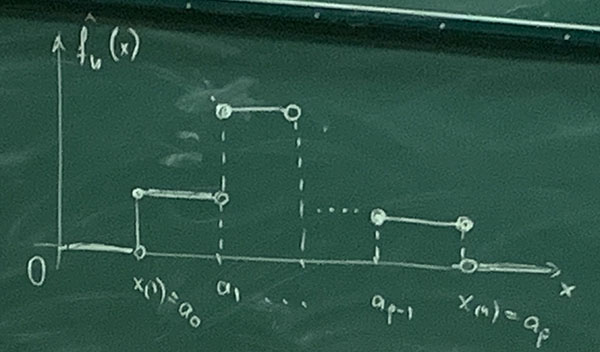
\includegraphics[scale=0.8]{img/hystogramm.jpg}
            \end{figure}

        \item
            \begin{equation*}
                \int_{-\infty}^{+\infty} \hat f_n(x) dx =
                \sum_{i=1}^p (\text{Площадь прямоугольников}) =
                \frac{n_1}{n\Delta} \cdot \Delta + ... +
                \frac{n_p}{n\Delta} \cdot \Delta = ... = 1
            \end{equation*}

        \item Эмпирическая плотность является выборочным аналогом
            функции плотности распределения вероятностей.
            Аналогично свойству выборочной функции распределения
            мгновенно доказывается, что для больший $n$

            \begin{equation*}
                \hat f_n(x) \approx f(x),
            \end{equation*}

            где $f$ -- теоретическая (<<истинная>>) фунцкия плотности
            распределения случайной величины $X$
    \end{enumerate}
\end{note}

\subsubsection{Полигон частот}

Предположим, что для выборки $X$ построена гистограмма.

\begin{defenition}
    Полигоном частот называется ломаная, звенья которой соединяют
    середины верхних сторон соседних прямоугольников гисторграммы.
\end{defenition}

\begin{figure}[H]
    \centering
    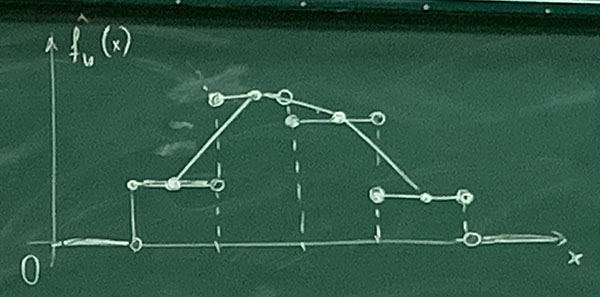
\includegraphics[scale=0.8]{img/polygon.jpg}
\end{figure}

\section{Точечные оценки}

\subsection{Основные понятия}

Рассмотрим 2-ю основную задачу математической статистики.

Дано: $X$ -- случайная величина, закон распределения которой известен
с точностью до вектора $\vec \Theta = (\Theta_1, ..., \Theta_r)$
неизвестных параметров (Это означает, что известен общий вид
закона распределения случайной величины $X$, но неизвестны значения
некоторых числовых параметров этого закона).

Требуется: оценить значение вектора $\vec \Theta$.

Для упрощения обозначений будем считать, что
$r = 1$, т.е. $\vec \Theta = (\Theta)$

\begin{defenition}
    Точечной оценкой параметра $\Theta$ называется статистика
    $\hat \Theta(\vec X)$, выборочное значение которой принимается
    в качестве значения этого параметра, то есть полагают

    \begin{equation*}
        \Theta := \hat \Theta (\vec x)
    \end{equation*}
\end{defenition}

\begin{example}
    \begin{enumerate}
        \item Пусть $X$ -- случайная величина, $m = MX$ -- неизвестно.
            Для оценки параметра $m$ можно предложить статистики:

            \begin{equation*}
                \hat m_1 (\vec X) = \overline{X} =
                \frac{1}{n} \sum_{i=1}^n X_i - \text{выборочное среднее}
            \end{equation*}

            \begin{equation*}
                \hat m_2 (\vec X) = \frac{X_{(1)} + X_{(n)}}{2}
            \end{equation*}

            \begin{equation*}
                \hat m_3 (\vec X) =
                \begin{cases}
                    X_{(\frac{n+1}{2})}, \text{ если n -- нечетное} \\
                    \frac{1}{2} \bigg[ X_{(\frac{n}{2})} +
                    X_{(\frac{n+2}{2})}\bigg], \text{ иначе} \\
                \end{cases}
            \end{equation*}

            \begin{equation*}
                \hat m_4 \big(\vec X\big) = \sin(\overline X)^2 +
                \sigma^2 \big(\vec X\big) \cdot
                \exp \big( -\overline X + X^2_{(1)} - X^{15}_{(n)} \big)
            \end{equation*}
    \end{enumerate}
\end{example}

Очевидно, что статистики
$\hat m_1, \hat m_2, \hat m_3$ из предыдущего примера будут
давать более или менее удовлетворительный результат, а последняя
статистика вряд ли будет давать что-то близкое к $m$. Тем не менее,
все эти статистики являются точечными оценками для $m$, так как
в определении ничего не сказано о том, что соответсвующая статистика
должна давать <<хорошие>> результаты. Дл исследования
качества построенной оценки используются характеристики:

\begin{enumerate}
    \item несмещенность
    \item состоятельность
    \item эффективность
\end{enumerate}

\begin{note}
    Из замечания не следует, что статистика $\hat \Theta$ должна
    принимать значения хоть сколько-нибудь близкие к теоретическому
    (<<истинному>>) значению параметра $\Theta$.
\end{note}

\subsection{Несмещенность точечной оценки}


\begin{defenition}
    Пусть $\hat \Theta(\vec X)$ -- точечная оценка неизвестного параметра
    $\Theta$.

    Оценка $\hat \Theta$ параметра $\Theta$ называется несмещенной, если
    ее математическое ожидание равно теоретическому значению неизвестного
    параметра, т.е.

    \begin{equation*}
        \exists M[\hat \Theta(\vec X)] = \Theta
    \end{equation*}
\end{defenition}

\begin{example}
    \begin{enumerate}
        \item Пусть $X$ -- случайная величина, $m=MX$ -- неизвестный
            параметр

            \begin{enumerate}
                \item Рассмотрим статистику

                    \begin{equation*}
                        \hat m_1 = \vec X
                    \end{equation*}

                    \begin{equation*}
                        M[\hat m_1] = M\bigg[\overline{X}\bigg] =
                        M[\frac{1}{n} \sum_{i=1}^n X_i] =
                        \frac{1}{n} \sum_{i=1}^n MX_i =
                    \frac{1}{n} \sum_{i=1}^n m = m
                    \end{equation*}

                    является несмещенной оценкой для $m$

                \item Рассмотрим статистику

                    \begin{equation*}
                        \hat m_2 = X_1
                    \end{equation*}

                    Тогда

                    \begin{equation*}
                        M[\hat m_2] = M[X_1] = MX = m
                    \end{equation*}

                    тоже несмещенная оценка
            \end{enumerate}

        \item $X$ -- случайная величина, $\exists MX, \exists DX = \sigma^2$

            Оказывается выборочная дисперсия

            \begin{equation*}
                \hat \sigma^2(\vec X) = \frac{1}{n} \sum_{i=1}^n
                (X_i - \overline{X} )^2
            \end{equation*}

            является смещенной оценкой для $\sigma^2$
    \end{enumerate}

    ФОТО
\end{example}

\begin{defenition}
    Статистика $\sigma^2$ называется направленной выборочной дисперсией
\end{defenition}

\subsection{Состоятельность точечной оценки}

\begin{defenition}
    Пусть

    \begin{enumerate}
        \item $X$ -- случайная величина, общий вид закона распределения
            которой известен
        \item $\Theta$ -- неизвестный параметр
        \item $\hat \Theta(\vec X)$ -- точечная оценка для $\Theta$
    \end{enumerate}

    Оценка $\hat \Theta(\vec X)$ параметра $\Theta$ называется
    состоятельной, если

    \begin{equation*}
        \hat \Theta(\vec X) \xrightarrow[n \to \infty]{P}  \Theta,
    \end{equation*}

    то есть

    \begin{equation*}
        \forall \varepsilon > 0 P\{|\hat \Theta(\vec X) -
        \Theta| > \varepsilon \} \xrightarrow[n \to \infty]{} 0
    \end{equation*}
\end{defenition}

\begin{example}
    Пусть

    \begin{enumerate}
        \item $X$ -- случайная величина
        \item $\exists MX = m$
        \item $\exists DX < \infty$
    \end{enumerate}

    Тогда $\hat m_1 = \overline{X}$ -- состоятельная оценка для $m$

    Доказательство:
    \begin{enumerate}
        \item Последовательность $X_1, X_2,...$ является
            последовательностью независимых одинаково распределенных
            случайных величин (см. определение случайной выборки)
        \item $MX_i = MX = m$
        \item $\exists DX < \infty$
    \end{enumerate}

    В соответствии со следствием ЗБЧ в форме Чебышева для одинаково
    распределенных случайных величин:

    \begin{equation*}
        \forall \varepsilon > 0 P\{ | \frac{1}{n} \sum_{i=1}^n X_i -
        m | > \varepsilon \} \xrightarrow[n \to \infty]{} 0,
    \end{equation*}

    То есть

    \begin{equation*}
        \overline{X} \xrightarrow[n \to \infty]{P} m
    \end{equation*}
\end{example}

\begin{note}
    Состоятельность оценки $\hat m_1 = \overline X$ математического
    ожидания можно доказать, не предполагая существования конечной
    дисперсии случайной величины X
\end{note}

\begin{example}
Пусть

    \begin{enumerate}
        \item $X\sim N(m,\sigma^2)$
        \item $\hat m_2(\vec X)=X_1$ -- точечная оценка для m
    \end{enumerate}

    Покажем, что $m_2$ не является состоятельной. 
    
    Доказательство:
    \begin{equation*}
        P\{|\hat m_2(\vec X)-m|>\varepsilon\}=P\{|X_1-m|>\varepsilon\}=\bigg|X_1\sim X,~~\text{то есть } f_{X_1}(x)=
        \frac{1}{\sqrt{2\pi }\sigma} e^{-\frac{(x-m)^2}{2\sigma^2}}\bigg|=\bigg|X_1-m\sim N(0,\sigma^2)\bigg|=
    \end{equation*}
    \begin{equation*}
        =\frac{1}{\sqrt{2\pi }\sigma} \int^\varepsilon_{-\varepsilon}e^{-\frac{t^2}{2\sigma^2}}dt=\underbrace{2\Phi_0\bigg(\frac{\varepsilon}{\sigma}\bigg)}_{\text{не зависит от } n}\ne 0 ~~(\text{при } n \to \infty)
    \end{equation*}

\end{example}

\begin{note}
    \begin{enumerate}
        \item Можно показать, что оценка

            \begin{equation*}
                S^2 (\vec X) = \frac{1}{n-1} \sum_{i=1}^n (X_i -
                \overline X)^2
            \end{equation*}

            Является состоятельной оценкой дисперсии случайной величины $X$,
            если у $X$ $\exists$ моменты до 4-го порядка включительно

        \item Более общо: можно показать, что если у случайной величины $X$
            $\exists$ начальный и центарльный моменты, то соответствующие
            выборочные аналоги являются их состоятельными оценками.
            При этом оценки моментов порядка $k \geq 2$ будут
            смещенными.
    \end{enumerate}
\end{note}

\subsection{Эффективность точечной оценки}

\begin{defenition}
    Пусть

    \begin{enumerate}
        \item $X$ -- случайная величина
        \item $\Theta$ неизвестный параметр закона распределения
            случайной величины $X$
        \item $\hat \Theta_1 (\vec X), \hat \Theta_2 (\vec X)$ --
            две несмещенные точечные оценки для $\Theta$
        \item $\exists D \hat \Theta, \exists D \hat \Theta_2$
    \end{enumerate}

    Оценка $\hat \Theta_2$ называется более эффективной, чем
    $\hat \Theta_1$, если

    \begin{equation*}
        D \hat \Theta_2 < D \hat \Theta_1
    \end{equation*}
\end{defenition}

\begin{defenition}
    Несмещенная оценка $\hat \Theta (\vec X)$ параметра $\Theta$ называется
    эффективной, если она обладает наименьшей дисперсией среди всех
    несмещенных оценок параметра $\Theta$.
\end{defenition}

\begin{note}
    Часто говорят об оценке, эффективной среди класса $H$ оценок
    параметра $\Theta$. Более точно, если все оценки из класса $H$
    являются несмещенными, то оценка $\tilde \Theta \in H$ называется
    эффективной в классе $H$, если она обладает наименьшей дисперсией среди
    всех лценок из $H$.
\end{note}

\begin{example}
    Пусть $X$ -- случайная величина. $m = MX$
    $H$ -- класс линейных оценок для $m$.

    Покажем, что $\hat m_1 (\vec X) = \overline{X}$ является
    эффективной оценкой в классе $H$.

    Решение:

    \begin{enumerate}
        \item Линейная оценка имеет вид:

            \begin{equation*}
                \hat \mu (\vec X) = \lambda_1 X_1 + ... + \lambda_n X_n
            \end{equation*}
    \end{enumerate}

    ФОТО
\end{example}

\begin{theorem}
    О единственности эффективной оценки

    Пусть

    \begin{enumerate}
        \item $\hat \Theta_1 (\vec X)$ и $\hat \Theta_2 (\vec X)$ --
            две эффективные оценки для параметра $\Theta$
    \end{enumerate}

    Тогда

    \begin{equation*}
        \hat \Theta_1 (\vec X) = \hat \Theta_2 (\vec X)
    \end{equation*}
\end{theorem}

\begin{note}
    $\hat \Theta_1$ и $\hat Theta_2$ является случайными величинами, потому
    равенство $\hat \Theta_1 (\vec X) = \hat \Theta_2 (\vec X)$ понимается:

    \begin{equation*}
        P \{ \vec X \in \{ \vec x : \vec \Theta_1 (\vec x) \ne
        \hat \Theta_2 (\vec x) \}\} = 0
    \end{equation*}
\end{note}
